\chapter{Gruppentheorie}

Es seien $G, H$ zwei Gruppen.

\begin{definition}
  Eine Abbildung $f \colon G \to H$ ist ein \emph{Gruppenhomomorphismus}, wenn $f(g_1 g_2) = f(g_1) f(g_2)$ für alle $g_1, g_2 \in G$ gilt.
\end{definition}

\begin{definition}
  Eine Teilmenge $H \subseteq G$ ist eine \emph{Untergruppe} von $G$, wenn $1 \in H$ gilt, und für alle $h, h_1, h_2 \in H$ auch $h^{-1} \in H$ und $h_1 h_2 \in H$ gelten.
  Dies wird dann mit $H \subgroup G$ notiert.
\end{definition}

Ist $H \subgroup G$ eine Untergruppe, so lässt sich die Verknüpfung von $G$ auf $H$ einschränken, wodurch $H$ ebenfalls wieder eine Gruppe ist.

\begin{example}
  Es ist $\groupcenter{G} = \{g \in G \suchthat \forall h \in G: gh = hg\} \subgroup G$ das \emph{Zentrum} von $G$.
\end{example}

\begin{definition}
  Ein Gruppenelement $g \in \groupcenter{G}$ ist \emph{zentral} in $G$.
\end{definition}

\begin{definition}
  Der \emph{Kern} eines Gruppenhomomorphismus $f \colon G \to H$ ist
  \[
              \ker(f)
    \defined  \{
                g \in G
              \suchthat
                f(g) = 1
              \}
    \subgroup G \,.
  \]
\end{definition}

\begin{definition}
  Zwei Gruppenelemente $g_1, g_2 \in G$ sind \emph{konjugiert \textup(zueinander\textup)}, wenn es ein $h \in G$ mit $h g_1 h^{-1} = g_2$ gibt.
  Zwei Untergruppen $H_1, H_2 \subgroup G$ sind \emph{konjugiert \textup(zueinander\textup)}, wenn es ein $g \in G$ mit $g H_1 g^{-1} = H_2$ gibt.
\end{definition}





\section{Nebenklassen und Satz von Lagrange}

Es sei $G$ eine Gruppe und $H \subgroup G$ eine Untergruppe.

\begin{definition}
  Für alle $a \in G$ ist $aH \defined \{ ah \suchthat h \in H \}$ die \emph{Linksnebenklasse von $a$ bezüglich $H$}, und $Ha \defined \{ ha \suchthat h \in H \}$ die \emph{Rechtsnebenklasse von $a$ bezüglich $H$}.
\end{definition}

Für alle $a \in G$ gilt dabei
\[
        aH = H
  \iff  a \in H
  \iff  Ha = H \,.
\]
Auf $G$ werden nun durch
\[
        a \sim_L b
  \iff  aH = bH
  \quad\text{und}\quad
        a \sim_R b
  \iff  Ha = Hb
\]
zwei Äquivalenzrelationen definiert.
Dabei gilt für alle $a, b \in G$, dass
\[
        a \sim_L b
  \iff  aH = bH
  \iff  b^{-1} a H = H
  \iff  b^{-1} a \in H
  \iff  a^{-1} b \in H \,,
\]
sowie analog
\[
        a \sim_R b
  \iff  Ha = Hb
  \iff  H = H b a^{-1}
  \iff  b a^{-1} \in H
  \iff  a b^{-1} \in H \,.
\]
Dabei ist $x = a^{-1} b$ das eindeutige Gruppenelement mit $a \cdot x = b$.
Es folgt somit, dass
\begin{align*}
      [a]_{\sim_L}
   =  \{ b \in G \suchthat a \sim_L b \}
  &=  \{ b \in G \suchthat a^{-1} b \in H \}  \\
  &=  \{ b \in G \suchthat \exists h \in H : ah = b \}
   =  \{ ah \suchthat h \in H \}
   =  aH \,,
\end{align*}
sowie analog, dass $[a]_{\sim_R} = Ha$.
Die Äquivalenzklassen von $\sim_L$ und $\sim_R$ sind also genau die Linksnebenklassen Rechtsnebenklassen bezüglich $H$, also verschobene Versionen von $H$ selbst.
Dabei ist für jedes $a \in H$ die Abbildung
\[
          H
  \to     aH \,,
  \quad   h
  \mapsto ah
\]
bijektiv, weshalb $\card{aH} = \card{H}$ gilt, sowie analog auch $\card{Ha} = \card{H}$.

Es ist nun $G$ die disjunkte Vereinigung der Äquivalenzklassen von $\sim_L$, d.h.\ $G$ zerfällt in disjunkte verschobene Versionen von $H$.
Ist $G$ endlich, so folgt somit, dass $\card{G}$ ein Vielfaches von $\card{H}$ ist.

\begin{definition}
  Die \emph{Ordnung} einer Gruppe $G$ ist $\ord{G} \defined \card{G}$.
\end{definition}

\begin{corollary}[Satz von Lagrange]
  Ist $G$ endlich, so gilt $\ord{H} \divides \ord{G}$.
\end{corollary}

\begin{definition}
  Es ist $G/H \defined G/{\sim_L} = \{aH \suchthat a \in H\}$ die Menge der Linksnebenklassen und $H \backslash G \defined G/{\sim_R} = \{Ha \suchthat a \in G\}$ die Menge der Rechtsnebenklassen.
\end{definition}

Für die Inversions-Abbildung $(-)^{-1} \colon G \to G$, $g \mapsto g^{-1}$ gilt
\[
    (aH)^{-1}
  = H^{-1} a^{-1}
  = H a^{-1} \,,
\]
weshalb $(-)^{-1}$ eine Bijektion $G/H \to H \backslash G$ induziert.
Es gibt deshalb gleich viele Links-\ und Rechtsnebenklassen, d.h.\ es gilt $\card{G/H} = \card{H \backslash G}$.

\begin{definition}
  Der \emph{Index} von $H$ in $G$ ist $\groupindex{G}{H} \defined \card{G/H} = \card{H \backslash G}$.
\end{definition}

\begin{corollary}
  Ist $G$ endlich, so gilt $\ord{G} = \ord{H} \groupindex{G}{H}$, sowie äquivalent $\groupindex{G}{H} = \ord{G}/{\ord{H}}$.
  Insbesondere ist auch $\groupindex{G}{H}$ ein Teiler von $\ord{G}$.
\end{corollary}

\begin{lemma}
  Für $K \subgroup H \subgroup G$ gilt $\groupindex{G}{K} = \groupindex{G}{H} \groupindex{H}{K}$.
\end{lemma}






\section{Normalteiler und Quotientengruppen}



\subsection{Definition von Normalteilern}

Für eine Untergruppe $N \subgroup G$ sind die folgenden Bedingungen äquivalent:

\begin{enumerate}
  \item
    Für alle $a \in G$ gilt $aN = Na$.
  \item
    Für alle $a \in G$ gilt $aNa^{-1} = N$.
  \item
    Für alle $a \in G$ gilt $aNa^{-1} \subseteq N$.
\end{enumerate}

\begin{definition}
  Eine Untergruppe $N \subgroup G$, die eine \textup(und damit alle\textup) der obigen Bedingungen erfüllt, ist \emph{normal}, bzw.\ ein \emph{Normalteiler}.
  Dies wird mit $N \normalgroup G$ notiert.
\end{definition}

\begin{example}
  \begin{enumerate}
    \item
      Ist $G$ abelsch, so ist jede Untergruppe $N \subgroup G$ normal.
    \item
      Für $N \normalgroup G$ und $H \subgroup G$ mit $N \subgroup H$ gilt auch $N \normalgroup H$
    \item
      Jede Untergruppe $N \subgroup G$ vom Index $\groupindex{G}{N} = 2$ ist normal.
    \item
      Für jeden Gruppenhomomorphismus $f \colon G \to H$ ist $\ker(f)$ ein Normalteiler in $G$.
      \begin{enumerate}
        \item
          Für alle $n \geq 0$ ist $A_n \defined \{\sigma \in S_n \suchthat \sign(\sigma) = 1\} \normalgroup S_n$.
        \item
          Für alle $n \geq 0$ ist $\sorthogonal{n} = \{A \in \orthogonal{n} \suchthat \det(A) = 1\} \normalgroup \orthogonal{n}$.
      \end{enumerate}
  \end{enumerate}
\end{example}

\begin{definition}
  Der \emph{Normalisator} einer Untergruppe $H \subgroup G$ ist
  \[
              \normalizer{G}{H}
    \defined  \{ g \in G \suchthat gHg^{-1} = H \} \,,
  \]
  d.h.\ $\normalizer{G}{H}$ ist die größte Untergruppe von $G$, in der $H$ normal ist.
\end{definition}




\subsection{Konstruktion von Quotientengruppen}

Ist $N \normalgroup G$ ein Normalteiler, so lässt sich auf $G/N$ durch
\[
            gN
  \cdot     hN
  \defined  (gh)N
\]
eine Gruppenstruktur definieren.

\begin{definition}
  Für $N \normalgroup G$ ist $G/N$ die \emph{Quotientengruppe} von $G$ nach $N$.
\end{definition}

Die Gruppenstruktur auf $G/N$ ist eindeutig dadurch bestimmt, dass die \emph{kanonische Projektion}
\[
            p
  \colon    G
  \to       G/N
  \quad     g
  \mapsto   \class{g}
  \defined  gN
\]
ein Gruppenhomomorphismus ist.
Dabei gilt $\ker(p) = N$.

\begin{corollary}
  Eine Untergruppe $N \subgroup G$ ist genau dann normal, wenn es einen Gruppenhomomorphismus $f \colon G \to H$ mit $\ker(f) = N$ gibt.
\end{corollary}

\begin{remark}
  Es handelt sich bei dem obigen Vorgehen um eine von mehrenen möglichen Vorgehensweisen, Quotientengruppen zu konstruieren.
  Inbesondere lassen sich Quotientengruppen auch ohne Verwendung von Nebenklassen konstruieren.
  Entscheident ist für die Quotientengruppe $G/N$ nur, dass die kanonische Projektion $p \colon G \to G/N$ ein Gruppenhomomorphismus mit $\ker(p) = N$ ist, welcher die folgende universelle Eigenschaft besitzt:
\end{remark}



\subsection{Universelle Eigenschaft der Quotientengruppe}

\begin{theorem}[Homomorphiesatz für Gruppen]
  Ist $f \colon G \to H$ ein Gruppenhomomorphismus mit $N \subseteq \ker(f)$, so induziert $f$ einen eindeutigen Gruppenhomomorphismus $\induced{f} \colon G/N \to H$ mit $f = \induced{f} \circ p$, d.h.\ so dass das folgende Diagramm kommutiert:
  \[
    \begin{tikzcd}
        G
        \arrow{rr}[above]{f}
        \arrow{dr}[below left]{p}
      & {}
      & H
      \\
        {}
      & G/N
        \arrow[dashed]{ru}[below right]{\induced{f}}
      & {}
    \end{tikzcd}
  \]
  In anderen Worten:
  Es ergibt sich eine Bijektion
  \begin{align*}
                            \{ \text{Gruppenhomo.\ $\induced{f} \colon G/N \to H$} \}
    &\xlongrightarrow{\sim} \{ \text{Gruppenhomo.\ $f \colon G \to H$ mit $N \subseteq \ker(f)$} \} \,,  \\
                            \induced{f}
    &\mapsto                \induced{f} \circ p \,.
  \end{align*}
\end{theorem}

\begin{corollary}[1.\ Isomorphiesatz]
  Jeder Gruppenhomomorphismus $f \colon G \to H$ induziert einen Isomorphismus
  \[
                            G/{\ker(f)}
    \xlongrightarrow{\sim}  \im(f) \,,
    \quad                   \class{g}
    \mapsto                 f(g) \,.
  \]
\end{corollary}

\begin{corollary}[2.\ Isomorphiesatz]
  Es seien $N, K \normalgroup G$ zwei Normalteiler mit $N \subgroup K$.
  Dann ist $K/N$ normal in $G/N$, und es gibt einen wohldefinierten Isomorphismus
  \[
                            (G/N)/(K/N)
    \xlongrightarrow{\sim}  G/K \,,
    \quad                   \class{ \class{g} }
    \mapsto                 \class{g} \,.
  \]
\end{corollary}

\begin{corollary}[3.\ Isomorphiesatz]
  Es sei $H \subgroup G$ eine Untergruppe und $N \normalgroup G$ eine normale Untergruppe.
  Dann ist $HN = \{hn \suchthat h \in H, n \in N\}$ eine Untergruppe von $G$, $H \cap N$ eine normale Untergruppe von $H$, und es gibt einen wohldefinierten Isomorphismus
  \[
                            H/(H \cap N)
    \xlongrightarrow{\sim}  HN/N \,,
    \quad                   \class{h}
    \mapsto                 \class{h} \,.
  \]
\end{corollary}



\subsection{Korrespondenz von (normalen) Untergruppen}

\begin{proposition}
  Es sei $N \normalgroup G$ eine normale Untergruppe und $p \colon G \to G/N$, $g \mapsto \class{g}$ die kanonische Projektion.
  \begin{enumerate}
    \item
      Es gibt eine 1:1-Korrespondenz von Untergruppen
      \begin{align*}
        \{ \text{Untergruppen $H \subgroup G$ mit $N \subgroup H$} \}
        &\xleftrightarrow{1:1}
        \{ \text{Untergruppen $H' \subgroup G/N$} \} \,,
        \\
        H
        &\longmapsto
        p(H)
        =
        H/N \,,
        \\
        p^{-1}(H')
        &\longmapsfrom
        H' \,.
      \end{align*}
    \item
      Es gibt eine eingeschränkte 1:1-Korrespondenz zwischen normalen Untergruppen
      \begin{align*}
        \{ \text{Normalteiler $K \normalgroup G$ mit $N \subgroup K$} \}
        &\xleftrightarrow{1:1}
        \{ \text{Normalteiler $K' \normalgroup G/N$} \} \,,
        \\
        K
        &\longmapsto
        p(K)
        =
        K/N \,,
        \\
        p^{-1}(K')
        &\longmapsfrom
        K' \,.
      \end{align*}
    \item
      Für jeden Normalteiler $K \normalgroup G$ mit $N \subgroup K$ gilt dabei für den zugehörigen Normalteiler $K' = p(K) = K/N$ nach dem 2.\ Isomorphiesatz, dass
      \[
              G/K
        \cong (G/N)/(K/N)
        \cong (G/N)/K' \,.
      \]
      Auf beiden Seiten der obigen 1:1-Korrespondenz erhält man somit \textup(bis auf Isomorphie\textup) die gleichen Quotientengruppen.
  \end{enumerate}
\end{proposition}





\section{Erzeugte Untergruppen}



\subsection{Definition erzeugter Untergruppen}

Es sei $G$ eine Gruppe und $S \subseteq G$ eine Teilmenge.
Für eine Untergruppe $H \subseteq G$ sind die folgenden Bedingungen äquivalent:

\begin{enumerate}
  \item
    Es ist $H$ die kleinste Untergruppe von $G$, die $S$ enthält, d.h.\ es gilt $S \subseteq H$, und für jede Untergruppe $K \subgroup G$ mit $S \subseteq K$ gilt $H \subgroup K$.
  \item
    Es gilt $H = \bigcap_{K \subgroup G, S \subseteq K} K$.
  \item
    Es gilt
    $
        H
      = \{
          s_1^{\varepsilon_1} \dotsm s_n^{\varepsilon_n}
        \suchthat
          n \in \Natural,
          s_i \in S,
          \varepsilon_i = \pm 1
        \}
    $.
\end{enumerate}

\begin{definition}
  Die Untergruppe $H$, die eine \textup(und damit alle\textup) der obigen Bedingungen erfüllt, ist die \emph{von $S$ erzeugte} Untergruppe, und wird mit $\generated{S}$ notiert.
  Es ist $S$ ein \emph{Erzeugendensystem} von $H$.
\end{definition}

\begin{example}
  \begin{enumerate}
    \item
      Die symmetrische Gruppe $S_n$ wird von der Menge der Transpositionen $\{ (i, j) \suchthat 1 \leq i \neq j \leq n \}$ erzeugt.
      Ein weiteres Erzeugendensystem ist die Menge der einfachen Transpositionen $\{ (i, i+1) \suchthat 1 \leq i < n \}$.
    \item
      Ist $K$ ein Körper, so wird die Gruppe $\GL{n}{K}$ von der Menge der Elementarmatrizen erzeugt.
  \end{enumerate}
\end{example}



\subsection{Klassifikation zyklischer Gruppen}

\begin{definition}
  Ein Gruppe $G$ \emph{zyklisch}, wenn es ein $g \in G$ mit $G = \generated{g}$ gibt.
\end{definition}

\begin{example}
  \begin{enumerate}
    \item
      Die Gruppe $\Integer$ ist zyklisch mit Erzeuger $1$.
    \item
      Wird $G$ von $g \in G$ zyklisch erzeugt, so wird für jeden Normalteiler $N \normalgroup G$ die Quotientengruppe $G/N$ von $\class{1}$ zyklisch erzeugt.
    \item
      Insbesondere ist für alle $n \in \Integer$ die Quotientengruppe $\Integer/n \defined \Integer/n\Integer = \Integer/\generated{n}$ zyklisch mit Erzeuger $\class{1} \in \Integer/n$.
    \item
      Ist $K$ ein Körper, so ist jede endliche Untergruppe $H \subgroup K^\times$ zyklisch.
      Inbesondere ist $K^\times$ zyklisch, wenn $K$ endlich ist.
  \end{enumerate}
\end{example}

Es gilt auch die Umkehrung der obigen Beispiele, d.h.\ jede zyklische Gruppe ist zu genau einer der Gruppen $\Integer/n$ mit $n \geq 0$ isomorph:

\begin{lemma}
\label{lemma: subgroups of Z}
  Jede Untergruppe $H \subgroup G$ ist von der Form $H = \generated{n} = n\Integer$ für ein eindeutiges $n \geq 0$.
  Für $H = \{0\}$ gilt $n = 0$, und sonst gilt $n = \min \{k > 0 \suchthat k \in H\}$.
\end{lemma}

Ist $G$ zyklisch mit Erzeuger $g \in G$, so ist die Abbildung
\[
          f
  \colon  \Integer
  \to     G \,,
  \quad   n
  \mapsto g^n
\]
ein surjektiver Gruppenhomomorphismus, und induziert somit einen Isomorphismus
\[
          \induced{f}
  \colon  \Integer/{\ker(f)}
  \to     G \,,
  \quad   \class{n}
  \mapsto g^n \,.
\]
Es gibt es eindeutiges $n \geq 0$ mit $\ker(f) = n\Integer$.
Gilt $n = 0$, so ist gilt $\Integer \cong G$, und $G$ ist unendlich.
Ansonsten gilt $n > 1$ und somit $G \cong \Integer/n$ mit $\ord{G} = n$.

\begin{corollary}[Klassifikation zyklischer Gruppen]
  Jede zyklische Gruppe $G$ ist zu genau einer der Gruppen $\Integer$, $\Integer/n$ mit $n \geq 1$ isomorph.
  Dabei gilt
  \[
          G
    \cong \begin{cases}
              \Integer
            & \text{falls $G$ unendlich ist} \,,
          \\
              \Integer/n
            & \text{falls $n = \ord{G}$ endlich ist} \,.
          \end{cases}
  \]
\end{corollary}

\begin{corollary}
  Untergruppen zyklischer Gruppen sind ebenfalls zyklisch.
\end{corollary}

\begin{definition}
  Für $g \in G$ ist $\ord{g} = \ord{\generated{g}}$ die \emph{Ordnung von $g$}.
\end{definition}

\begin{lemma}
  Es sei $g \in G$.
  \begin{enumerate}
    \item
      Ist $G$ eine endliche Gruppe, so gilt $\ord{g} \divides \ord{G}$.
      Insbesondere gilt $g^{\ord{G}} = 1$.
    \item
      Hat $g$ endliche Ordnung, so gilt $\ord{g} = \min \{ n \geq 1 \suchthat g^n = 1 \}$.
  \end{enumerate}
\end{lemma}

\begin{example}[Gruppen von Ordnung $p$]
  Es sei $p$ prim und $G$ eine Gruppe von Ordnung $\ord{G} = p$.
  Dann gibt es ein nicht-triviales Element $g \in G$.
  Dann ist $\ord{g} \neq 1$ ein Teiler von $\ord{G} = p$, und somit $\ord{g} = \ord{G}$, also $\generated{g} = G$.
  Somit ist $G$ zyklisch, also $G \cong \Integer/p$.
\end{example}

%TODO: Exercise: subgroups of S3





\section{Gruppenwirkungen}



\subsection{Grundlegende Definitionen}

\begin{definition}
  Es sei $G$ eine Gruppe und $X$ eine Menge.
  Eine \emph{\textup(Gruppen\textup)wirkung} von $G$ auf $X$ ist eine Abbildung $G \times X \to X$, $(g,x) \mapsto g.x$ mit $1.x = x$ und $g.(h.x) = (gh).x$ für alle $g, h \in G$, $x \in X$.
  
  Eine \emph{$G$-Menge} ist eine Menge $X$ zusammen mit einer Wirkung von $G$ auf $X$.
\end{definition}

\noindent
\begin{minipage}[t]{\textwidth}
Es sei $G$ eine Gruppe und $X$ eine Menge.
\begin{itemize}
  \item
    Wirkt $G$ auf $X$, so ist für jedes $g \in G$ die Abbildung $\lambda_g \colon X \to X$, $x \mapsto g.x$ eine Bijektion, und die Abbildung $G \to \symmetric{X}$, $g \mapsto \lambda_g$ ist ein Gruppenhomomorphismus.
  \item
    Ist andererseits $\varphi \colon G \to \symmetric{X}$ ein Gruppenhomomorphismus, so wird durch $g.x \defined \varphi(g)(x)$ eine Wirkung von $G$ auf $X$ definiert.
\end{itemize}
Diese beiden Konstruktionen sind invers zueinander, weshalb eine Wirkung von $G$ auf $X$ einem Gruppenhomomorphismus $G \to \symmetric{X}$ entspricht.
\end{minipage}

\begin{definition}
  Es sei $X$ eine $G$-Menge und $x \in X$.
  \begin{enumerate}
    \item
      Die \emph{$G$-Bahn} von $x$ ist $G.x \defined \{g.x \suchthat g \in G\}$.
    \item
      Es ist $X/G \defined \{G.x \suchthat x \in X\}$ die Menge der $G$-Bahnen.
    \item
      Der \emph{Stabilisator} von $x$ ist $G_x \defined \{g \in G \suchthat g.x = x\}$.
    \item
      Die \emph{Fixpunktmenge} von $X$ ist $X^G \defined \{x \in X \suchthat \forall g \in G: g.x = x\}$.
  \end{enumerate}
\end{definition}

\begin{lemma}
  Es sei $X$ eine $G$-Menge.
  \begin{enumerate}
    \item
      Für alle $x \in X$ ist $G_x \subgroup G$ eine Untergruppe.
    \item
      Für alle $g \in G$, $x \in X$ gilt $G_{g.x} = g G_x g^{-1}$.
  \end{enumerate}
\end{lemma}

\begin{example}
  Die Gruppe $\GL{n}{K}$ wirkt auf dem Vektorraum $K^n$ durch $A.x \defined Ax$ für alle $A \in \GL{n}{K}$, $x \in K^n$.
  Für alle $x, y \in K^n$ mit $x, y \neq 0$ gibt es ein $A \in \GL{n}{K}$ mit $Ax = y$, weshalb diese Gruppenwirkung zwei Bahnen besitzt:
  $\{0\}$ und $K^n \smallsetminus \{0\}$.
  Insbesondere ist im Allgemeinen $0$ der einzige Fixpunkt dieser Wirkung;
  einzige Ausnahme ist der Fall $K = \Finite_2$, $n = 1$, dann sind beide Elemente Fixpunkte.
  Der Stabilisator des Standardbasisvektors $e_1$ ist die Untergruppe
  \[
              H
    \defined  \left\{
                \begin{pmatrix}
                  1 & * \\
                  0 & A
                \end{pmatrix}
              \suchthat*
                A \in \GL{n-1}{K}
              \right\} \,;
  \]
  der Stabilisator eines beliebigen Vektors $x \in K^n$, $x \neq 0$ ist konjugiert zu $H$.
\end{example}

\begin{definition}
  Es sei $X$ eine $G$-Menge.
  \begin{enumerate}
    \item
      Die Wirkung von $G$ auf $X$ ist \emph{transitiv}, wenn es für alle $x, y \in X$ ein $g \in G$ mit $g.x = y$ gibt.
    \item
      Die Wirkung von $G$ auf $X$ ist \emph{treu}, wenn es für alle $g, h \in G$ aus
      \[
        \text{$g.x = h.x$ für alle $x \in X$}
      \]
      folgt, dass $g = h$ gilt.
  \end{enumerate}
\end{definition}

\begin{remark}
  Eine Wirkung von $G$ auf $X$ ist genau dann treu, wenn der zugehörige Gruppenhomomorphismus $G \to \symmetric{X}$ injektiv ist.
\end{remark}

\begin{example}
  Die symmetrische Gruppe $S_n$ wirkt auf der Menge $X \defined \{1, \dotsc, n\}$ durch $\sigma.i \defined \sigma(i)$ für alle $\sigma \in S_n$, $i \in X$.
  Dies Wirkung ist transitiv und treu.
  Der zugehörige Gruppenhomomorphismus $S_n \to \symmetric{X} = S_n$ ist die Identität $\id_{S_n}$.
  Der Stabilisator von $i \in X$ ist $\{ \sigma \in S_n \suchthat \sigma(i) = i \} \cong S_{n-1}$.
\end{example}

\begin{example}
  Jede Gruppe $G$ wirkt auf sich selbst, d.h.\ auf $X \defined G$, auf zwei Weisen:
  \begin{enumerate}
    \item
      Die Gruppe $G$ wirkt auf sich selbst durch Linksmultiplikation, d.h.\ durch $g.x \defined gx$ für alle $g \in G$, $x \in X$.
      Diese Wirkung ist transitiv und treu, und für jedes $x \in X$ ist der Stabilisator $G_x$ trivial.
      
      Man bemerke, dass diese treue Wirkung einem injektiven Gruppenhomomorphismus $G \hookrightarrow \symmetric{X}$ entspricht, durch den sich $G$ als eine Untergruppe der symmetrischen Gruppe $\symmetric{X}$ auffassen lässt.
      Dies ist der \emph{Satz von Cayley}:
      Jede Gruppe ist isomorph zu einer Gruppe von Permutationen.
    \item
      Die Gruppe $G$ wirkt auf sich selbst durch Konjugation, d.h.\ für alle $g \in G$, $x \in X$ ist $g.x \defined gxg^{-1}$.
      Die Bahnen dieser Wirkung sind die \emph{Konjugationsklassen} von $G$.
      Für alle $g \in G$ $x \in X$ gilt
      \[
          g.x
        = x
        \iff
          gxg^{-1}
        = x
        \iff
          gx
        = xg \;
      \]
      die Fixpunktmenge $X^G$ dieser Wirkung ist deshalb das Zentrum $\groupcenter{G}$, und für jedes $x \in X$ ist $G_x = \{g \in G \suchthat gx = xg\} \eqqcolon \centralizer{G}{x}$ der \emph{Zentralisator} von $x$;
      dies ist die größte Untergruppe von $G$, in der $x$ zentral ist.
  \end{enumerate}
\end{example}



\subsection{Die Bahnenformel}

Es sei $X$ eine $G$-Menge.
Durch
\[
        x \sim y
  \iff  \exists g \in G: g.x = y
\]
wird eine Äquivalenzrelation auf $X$ definiert.
Für alle $x \in X$ gilt dann $[x]_{\sim} = G.x$.
Je zwei Bahnen $G.x$ und $G.y$ sind also entweder gleich oder disjunkt, und $X$ ist die disjunkte Vereinigung der $G$-Bahnen.
Ist $(x_i)_{i \in I}$ ein Repräsentantensystem der $G$-Bahnen von $X$, so gilt deshalb
\begin{equation}
\label{equation: orbit formula alpha}
    \card{X}
  = \sum_{i \in I} \card{G.x_i}
  = \card*{X^G} + \sum_{\substack{i \in I \\ x_i \notin X^G}} \card{G.x_i} \,.
\end{equation}
Für jedes $x \in X$ ist dabei die Abbildung $G \to G.x$, $g \mapsto g.x$ surjektiv, und es gilt
\[
        g.x = h.x
  \iff  h^{-1}g.x = x
  \iff  h^{-1} g \in G_x
  \iff  g G_x = h G_x \,.
\]

\begin{corollary}
  \label{corollary: classification of transitive G-sets}
  Für jedes $x \in G$ ist die Abbildung
  \[
            G/G_x
    \to     G.x \,,
    \quad   g G_x
    \mapsto g.x
  \]
  eine wolhdefinierte Bijektion.
  Insbesondere gilt $\card{G.x} = \card{G/G_x} = \groupindex{G}{G_x}$.
\end{corollary}

\begin{remark}
  Man bemerke, dass somit $\card{G.x}$ stets ein Teiler von $\card{G}$ ist!
\end{remark}

% \begin{example}
%   Ist $H \subgroup G$ eine Untergruppe, so wirkt $G$ auf der Menge der Linksnebenklassen $G/H$ durch $g.(g'H) \defined (gg')H$ für alle $g \in G$, $g'H \in G/H$.
%   Diese Wirkung ist transitiv, und der Stabilisator der Nebenklasse $H = 1H \in G/H$ ist
%   \[
%       G_H
%     = \{ g \in G \suchthat g.H = H \}
%     = \{ g \in G \suchthat gH = H \}
%     = H \,.
%   \]
%   Die induzierte Bijektion
%   \[
%             G/H
%     \to     G.H
%     =       G/H \,,
%     \quad   gH
%     \mapsto g.H
%     =       gH
%   \]
%   ist die Identität.
% \end{example}

Durch Lemma~\ref{corollary: classification of transitive G-sets} lässt sich Gleichung~\eqref{equation: orbit formula alpha} zu
\[
    \card{X}
  = \sum_{i \in I} \groupindex{G}{G_{x_i}}
  = \card*{X^G} + \sum_{\substack{i \in I \\ x_i \notin X^G}} \groupindex{G}{G_{x_i}} \,
\]
umschreiben.

\begin{corollary}[Bahnenformel]
  Ist $X$ eine $G$-Menge und $(x_i)_{i \in I}$ ein Repräsentantensystem der $G$-Bahnen von $X$, so gilt
  \[
      \card{X}
    =   \card*{X^G}
      + \sum_{\substack{i \in I \\ x_i \notin X^G}} \groupindex{G}{G_{x_i}}.
  \]
\end{corollary}










\pagebreak










\section{\texorpdfstring{$p$}{p}-Gruppen und Sylowsätze}

Es sei $G$ eine endliche Gruppe und $p$ prim.

\begin{definition}
  Gilt $\ord{G} = p^n$ für ein $n \in \Natural$, so ist $G$ eine \emph{$p$-Gruppe}.
\end{definition}

\begin{example}
  \begin{enumerate}
    \item
      Es ist $\Integer/p$ bis auf Isomorphie die einzige Gruppe der Ordnung $p$.
    \item
      Jede Gruppe der Ordnung $p^2$ ist abelsch, und entweder isomorph zu $\Integer/p^2$ oder zu $\Integer/p \times \Integer/p$.
    \item
      Die Heisenberg-Gruppe
      \[
                  H
        \defined  \left\{
                    \begin{pmatrix}
                      1 & a & b \\
                        & 1 & c \\
                        &   & 1
                    \end{pmatrix}
                  \suchthat*
                    a, b, c \in \Finite_p
                  \right\}
      \]
      ist eine nicht abelsche Gruppe der Ordnung $p^3$.
  \end{enumerate}
\end{example}

\begin{lemma}
  Ist $G \neq 1$ eine nicht-triviale $p$-Gruppe, so gilt auch $\groupcenter{G} \neq 1$.
\end{lemma}

\begin{corollary}
  Ist $G$ eine $p$-Gruppe, so besitzt besitzt $G$ eine Normalenreihe
  \[
                  G_0
    =             \{ 1 \}
    \normalgroup  G_1
    \normalgroup  G_2
    \normalgroup  G_3
    \normalgroup  \dotsb
    \normalgroup  G_n
    =             G
  \]
  mit Quotienten $G_i / G_{i-1} \cong \Integer/p$ für alle $i = 1, \dotsc, n$, d.h.\ es gilt $\card{G_r} = p^r$ für alle $r$.
\end{corollary}

\begin{definition}
  Eine \emph{$p$-Sylow\-unter\-gruppe} von $G$ eine $p$-Untergruppe $S \subgroup G$ mit $\ord{S} = p^r$ und $p \notdivides \groupindex{G}{S}$, d.h.\ es gilt $\ord{G} = p^r m$ mit $p \notdivides m$.
\end{definition}

\begin{theorem}[Sylowsätze]
  Es gelte $G = p^r m$ mit $p \notdivides m$.
  \begin{enumerate}
    \item
      Jede $p$-Untergruppe $H \subgroup G$ ist in einer $p$-Sylowuntergruppe von $G$ enthalten.
      Inbesondere ergibt sich für $H = \{1\}$, dass $G$ eine $p$-Sylowuntergruppe besitzt.
    \item
      Je zwei $p$-Sylowuntergruppen $S, S' \subseteq G$ sind konjugiert zueinander, d.h.\ es gibt ein $g \in G$ mit $g S g^{-1} = S'$.
    \item
      Bezeichnet $n_p$ die Anzahl der $p$-Sylowuntergruppen von $G$, so gilt
      \[
                n_p
        \equiv  1
        \pmod{p}
        \quad\text{und}\quad
        n_p \divides m \,.
      \]
  \end{enumerate}
\end{theorem}

\begin{corollary}
  Eine $p$-Sylowuntergruppe $S \subgroup G$ ist genau dann normal, wenn $n_p = 1$.
\end{corollary}

\begin{corollary}
  Ist $G$ abelsch, so besitzt $G$ eine eindeutige $p$-Sylowuntergruppe.
\end{corollary}





\section{Klassifikation endlicher abelscher Gruppen}

Es sei $G$ eine endliche abelsche Gruppe.

\begin{theorem}
  Für jede Primzahl $p$ sei $S_p$ die eindeutige $p$-Sylowuntergruppe von $G$.
  Sind $p_1, \dotsc, p_n$ die Primfaktoren von $\card{G}$, so ist die Abbildung
  \[
                            S_{p_1} \times \dotsb \times S_{p_r}
    \xlongrightarrow{\sim}  G \,,
    \quad                   (g_1, \dotsc, g_r)
    \mapsto                 g_1 \dotsm g_r
  \]
  ein Isomorphismus.
\end{theorem}

\begin{proposition}
  Es sei $p$ prim.
  Jede abelsche $p$-Gruppe $G$ ist isomorph zu einem Produkt zyklischer $p$-Gruppen, d.h.\ es gilt
  \[
          G
    \cong \Integer/p^{n_1} \times \dotsm \times \Integer/p^{n_r}
  \]
  mit $n_1, \dotsc, n_r \geq 1$.
\end{proposition}

\begin{corollary}[Klassifikation endlicher abelscher Gruppen]
  Jede endliche abelsche Gruppe ist isomorph zu einem Produkt zyklischer $p$-Gruppen, d.h.\ es gilt
  \[
          G
    \cong \Integer/p_1^{n_1} \times \dotsm \times \Integer/p_r^{n_r}
  \]
  mit $p_1, \dotsc, p_r$ prim und $n_1, \dotsc, n_r \geq 1$.
\end{corollary}

Man bemerke, dass dabei $\card{G} = p_1^{n_1} \dotsm p_r^{n_r}$ gilt.

\begin{remark}
  Tatsächlich ist diese Zerlegung bereits eindeutig bis auf Permutation der Faktoren, d.h.\ die Paare $(p_1, n_1), \dotsc, (p_r, n_r)$ sind eindeutig bis auf Permuation.
  Diese Eindeutigkeit wurde in der Vorlesung allerdings nicht gezeigt.
\end{remark}





\section{Beispiel: Die Diedergruppe \texorpdfstring{$D_n$}{D\_n}}

Es sei $n \geq 3$.
Die \emph{Diedergruppe} $D_n$ ist die Symmetriegruppe des regelmäßigen $n$-Ecks.
\begin{center}
  \[
    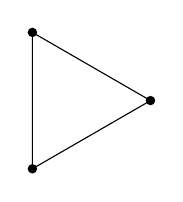
\begin{tikzpicture}
    % n = 3
      \draw (0:1)
      \foreach \x in {120, 240, 360} {
        -- (\x:1)
      };
      \foreach \x in {120, 240, 360} {
        \fill[black] (\x:1) circle (0.06);
      }
    \end{tikzpicture}
    \hspace{3em}
    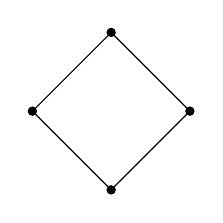
\begin{tikzpicture}
    % n = 4
      \draw (0:1)
      \foreach \x in {90, 180, 270, 360} {
        -- (\x:1)
      };
      \foreach \x in {90, 180, 270, 360} {
        \fill[black] (\x:1) circle (0.06);
      }
    \end{tikzpicture}
    \hspace{3em}
    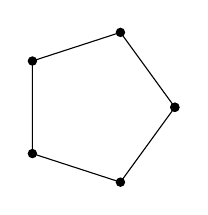
\begin{tikzpicture}
    % n = 5
      \draw (0:1)
      \foreach \x in {72,144,...,360} {
        -- (\x:1)
      };
      \foreach \x in {0, 72, ..., 360} {
        \fill[black] (\x:1) circle (0.06);
      }
    \end{tikzpicture}
    \hspace{3em}
    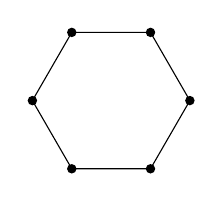
\begin{tikzpicture}
    % n = 6
      \draw (0:1)
      \foreach \x in {60, 120, ..., 360} {
        -- (\x:1)
      };
      \foreach \x in {60, 120, ..., 360} {
        \fill[black] (\x:1) circle (0.06);
      }
    \end{tikzpicture}
  \]
  Ein regelmäßiges $n$-Eck für $n = 3, 4, 5, 6$.
\end{center}
Die Gruppe $D_n$ besteht also aus zwei Arten von Elementen:
\begin{itemize}
  \item
    Den Rotationen um Vielfache des Winkels $2\pi/n$.
    Dies sind insgesamt $n$ Rotationen.
    \[
      % triangle
      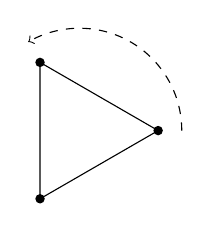
\begin{tikzpicture}
        \draw (0:1)
        \foreach \x in {120, 240, 360} {
          -- (\x:1)
        };
        \foreach \x in {120, 240, 360} {
          \fill[black] (\x:1) circle (0.06);
        }
        \draw[->,dashed] (0:1.3) arc[radius=1.3, start angle=0, end angle=120];
      \end{tikzpicture}
      \hspace{5em}
      % square
      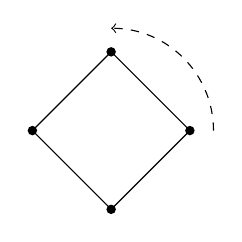
\begin{tikzpicture}
        \draw (0:1)
        \foreach \x in {90, 180, 270, 360} {
          -- (\x:1)
        };
        \foreach \x in {90, 180, 270, 360} {
          \fill[black] (\x:1) circle (0.06);
        }
        \draw[->,dashed] (0:1.3) arc[radius=1.3, start angle=0, end angle=90];
      \end{tikzpicture}
      \hspace{5em}
      % pentagon
      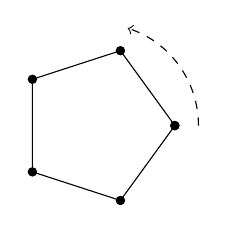
\begin{tikzpicture}
        \draw (0:1)
        \foreach \x in {0, 72, ..., 360} {
          -- (\x:1)
        };
        \foreach \x in {0, 72, ..., 360} {
          \fill[black] (\x:1) circle (0.06);
        }
        \draw[->,dashed] (0:1.3) arc[radius=1.3, start angle=0, end angle=72];
      \end{tikzpicture}
    \]
  \item
    Es gibt $n$ Spiegelungen in $D_n$:
    \begin{itemize}
      \item
        Ist $n$ ungerade, so gehen die Spiegelungsachsen durch jeweils einen der Eckpunkte sowie den Mittelpunkt der gegenüberliegenden Achse:
        \[
          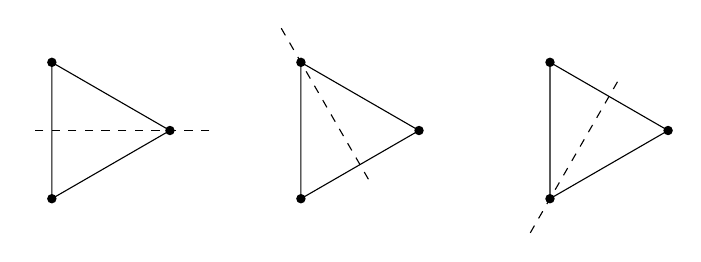
\begin{tikzpicture}
            % first triangle
            \draw (0:1)
            \foreach \x in {120, 240, 360} {
              -- (\x:1)
            };
            \foreach \x in {120, 240, 360} {
              \fill[black] (\x:1) circle (0.06);
            }
            \draw[dashed] (0:1.5) -- (180:0.8);
            % second triangle
            \draw ([xshift=9em]0:1)
            \foreach \x in {120, 240, 360} {
              -- ([xshift=9em]\x:1)
            };
            \foreach \x in {120, 240, 360} {
              \fill[black] ([xshift=9em]\x:1) circle (0.06);
            }
            \draw[dashed] ([xshift=9em]120:1.5) -- ([xshift=9em]300:0.8);
            % third triangle
            \draw ([xshift=18em]0:1)
            \foreach \x in {120, 240, 360} {
              -- ([xshift=18em]\x:1)
            };
            \foreach \x in {120, 240, 360} {
              \fill[black] ([xshift=18em]\x:1) circle (0.06);
            }
            \draw[dashed] ([xshift=18em]240:1.5) -- ([xshift=18em]60:0.8);
          \end{tikzpicture}
          \hspace{5em}
        \]
      \item
        Ist $n$ gerade, so gibt es $n/2$ Spiegelungen, deren Achsen durch einen der Eckpunkte sowie den gegenüberliegenden Eckpunkt gehen, sowie $n/2$ Spiegelungen, die durch einen der Seitenmittelpunkte sowie den gegenüberliegenden Seitenmittelpunkt gehen:
        \[
          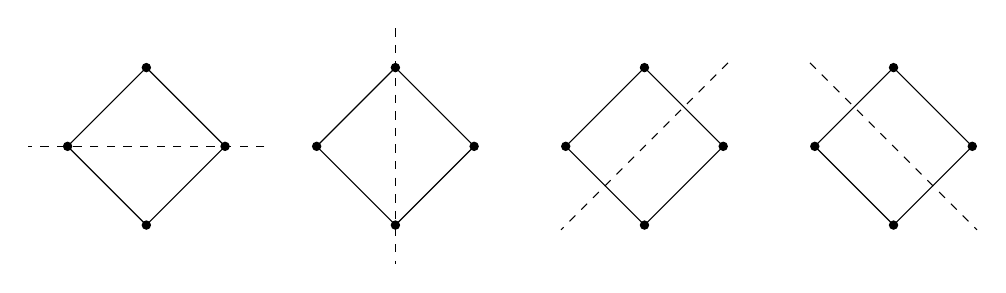
\begin{tikzpicture}
          % first square
            \draw (0:1)
            \foreach \x in {90, 180, 270, 360} {
              -- (\x:1)
            };
            \foreach \x in {90, 180, 270, 360} {
              \fill[black] (\x:1) circle (0.06);
            }
            \draw[dashed] (0:1.5) -- (180:1.5);
          % second square
            \draw ([xshift=9em]0:1)
            \foreach \x in {90, 180, 270, 360} {
              -- ([xshift=9em]\x:1)
            };
            \foreach \x in {90, 180, 270, 360} {
              \fill[black] ([xshift=9em]\x:1) circle (0.06);
            }
            \draw[dashed] ([xshift=9em]90:1.5) -- ([xshift=9em]270:1.5);
          % third square
            \draw ([xshift=27em]0:1)
            \foreach \x in {90, 180, 270, 360} {
              -- ([xshift=27em]\x:1)
            };
            \foreach \x in {90, 180, 270, 360} {
              \fill[black] ([xshift=27em]\x:1) circle (0.06);
            }
            \draw[dashed] ([xshift=27em]135:1.5) -- ([xshift=27em]315:1.5);
          % fourth square
            \draw ([xshift=18em]0:1)
            \foreach \x in {90, 180, 270, 360} {
              -- ([xshift=18em]\x:1)
            };
            \foreach \x in {90, 180, 270, 360} {
              \fill[black] ([xshift=18em]\x:1) circle (0.06);
            }
            \draw[dashed] ([xshift=18em]45:1.5) -- ([xshift=18em]225:1.5);
          \end{tikzpicture}
        \]
    \end{itemize}
\end{itemize}

Ingesamt besteht die Gruppe $D_n$ somit aus $2n$ Elementen, davon $n$ Rotationen und $n$ Spiegelungen.
Jedes $\sigma \in D_n$ permutiert die Eckpunkte des regelmäßigen $n$-Ecks, dabei ist die Wirkung von $\sigma$ auf dem gesamten $n$-Eck bereits eindeutig durch die Wirkung auf den Eckpunkten bestimmt.
Indem man die Eckpunkte mit $1, \dotsc, n$ durchnummeriert, lässt sich also $D_n$ mit einer Untergruppe von $S_n$ identifizieren.

\begin{example}
  Es sei $n = 4$.
  \[
    \begin{tikzpicture}[scale=1.5]
      \draw (0:1)
      \foreach \x in {90, 180, 270, 360} {
        -- (\x:1)
      };
      \foreach \i in {1,2,3,4} {
        \fill[black] (90*\i:1) circle (0.06);
        \draw (90*\i:1.25) node {\i};
      }
    \end{tikzpicture}
  \]
  \begin{center}
    \begin{tabular}{|c|c|}
      \hline
        \begin{tabular}{c}
          Spiegelungen mit Achse  \\
          durch die Eckpunkte
        \end{tabular}
      & $(1, 3)$ und $(2, 4)$
      \\
      \hline
        \begin{tabular}{c}
          Spiegelungen mit Achse  \\
          durch die Seitenmittelpunkte
        \end{tabular}
      & $(1,2)(3,4)$ und $(1,4)(2,3)$
      \\
      \hline
        \begin{tabular}{c}
          Rotationen um \\
          $0^\circ$, $90^\circ$, $180^\circ$, $270^\circ$
        \end{tabular}
      & $\id$, $(1,2,3,4)$, $(1,3)(2,4)$, $(4,3,2,1)$
      \\
        \hline
    \end{tabular}
  \end{center}
%   Fasst man auf diese Weise $D_4$ als Untergruppe on $S_4$ auf, so folgt aus $\card{D_4} = 8 = 2^3$, dass $D_4$ eine $2$-Sylowuntergruppe von $S_4$ ist.
\end{example}

Für $n = 3$ gilt $\card{D_3} = 2 \cdot 3 = 6 = 3! = \card{S_3}$, weshalb die Einbettung $D_3 \hookrightarrow S_3$ bereits ein Isomorphismus ist.

\begin{corollary}
  Es gilt $D_3 \cong S_3$.
\end{corollary}

\begin{proposition}
  Es seien $n, m \geq 3$.
  \begin{enumerate}
    \item
      Gilt $n \divides m$, so gibt es eine Einbettung $D_n \hookrightarrow D_m$:
      \[
        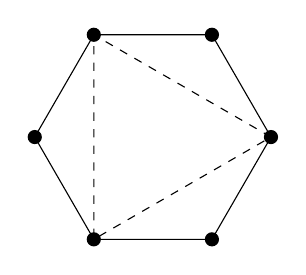
\begin{tikzpicture}[scale=1.5]
          % hexagon
          \draw (0:1)
          \foreach \x in {60, 120, ..., 360} {
            -- (\x:1)
          };
          \foreach \x in {60, 120, ..., 360} {
            \fill[black] (\x:1) circle (0.06);
          }
          % triangle
          \draw[dashed] (0:1)
          \foreach \x in {120, 240, 360} {
            -- (\x:1)
          };
        \end{tikzpicture}
      \]

    \item
      Gilt $n = 2m$ mit $m$ ungerade, so gilt $D_n \cong D_m \times (\Integer/2)$.
  \end{enumerate}
\end{proposition}





